\documentclass{ctexart}
\usepackage[a4paper, margin=3cm]{geometry}

\usepackage{amsmath}
\usepackage{amssymb}
\usepackage{minted}
\usepackage{graphics}
\usepackage{graphicx}
\usepackage{todonotes}

\title{网络安全工程与实现 HW4 设计文档}
\author{刘晓义 2017011426, 任乐图}

\begin{document}
  \maketitle

  \tableofcontents

  \section{协议设计}

  设计为一个 4 层代理,传递 TCP / UDP 协议的内容。

  \subsection{攻击模型}

  在我们考虑的攻击模型中,假设攻击者具有以下能力/信息:

  \begin{itemize}
    \item 可能位于链路中间人上。
    \item 拥有小于2022年地球上全部计算资源总和以内的计算能力。
    \item 可能拥有用户权限。在这种情况下,需要防止的攻击是针对其他用户的。特别地,这意味着握手包不能使用 Pre-shared key + 对称加密。
  \end{itemize}

  假设攻击者\textbf{没有}以下能力/信息
  \begin{itemize}
    \item 我们假设攻击者无法获得服务器和客户端进程本身的任何信息。这包括在主机上测量的执行时间、随机数源等。原因是我们不太懂 Time-invariant cryptography(笑)。
    \item 对于上游链路:
    \begin{itemize}
      \item 在考虑攻击者破解消息内容,或者根据侧信道阻断(例如发送 Reset)的时候,我们假设攻击者不控制下游服务器,或无法监听下游链路。否则如果我们希望保持低延迟,攻击者在时间序列上可以很容易推断相关性。
      \item 在考虑攻击者对消息篡改的能力时,我们假设攻击者在下游链路上只能有监听能力,但无法篡改。否则服务器就无法保证支持所有的连接(例如明文 HTTP)。
      \item 特别地,在考虑攻击者尝试破解密钥时,我们\textbf{允许}攻击者在下游依旧有监听、篡改消息的能力。因此我们需要选择保证 CCA2-resistent 的 Cipher。
    \end{itemize}
  \end{itemize}

  \subsection{目标}

  我们希望能够达成的保护包括:

  \begin{itemize}
    \item 保证信息的保密性 (Confidentiality),权威性(Authenticity)和完整性(Integrity)。更细节的:
    \begin{itemize}
      \item 我们需要识别对消息的篡改,重放
      \item 我们需要保证攻击者无法得到消息内容
      \item 我们需要保证攻击者无法获取(自己之前未掌握的)密钥,包括 Session key 和 User key。
      \item 攻击者无法识别用户
    \end{itemize}
    \item 在可用性上,尽量减小协议被识别的可能,并在被阻断之后可以在对上层连接透明地情况下重连。但在攻击者持有用户帐号的时候,我们\textbf{允许}攻击者对于服务器端口的识别,以及根据这一信息对于客户端连接的识别。
  \end{itemize}

  为了简化客户端的实现,客户端启动的时候指定一个代理出口连接的 IP 、四层协议和端口,如果想连接到其他地方需要再启动新的客户端,类似 socat 的工作方法。这只是为了方便客户端的实现,使得我们不用设计上游应用(curl,浏览器)和客户端之间的协议。\textbf{服务端和协议设计并无这一限制。}

  \vspace*{1em}

  为了实现方便,我们不考虑的东西包括:

  \begin{itemize}
    \item 细节的性能考量。我们希望协议能有最小的 Overhead,但有些时候为了设计简单,我们会传递较多的包和元信息。
    \item 连接级别的向前安全性。我们不会在一个连接内修改 Session key。当然,不同连接还是会使用不同的 Session key。
    \item 对于 ECDHE 过程的识别。如果需要伪装这部分连接,可能最好的办法是完全实现一个内容随机的 TLS ClientHello。这本身不是技术上的困难,只是实现很麻烦,所以我们忽略了这一部分。在 ECDHE 之后,剩余的握手和消息传递协议设计都会对侧信道识别有所考虑。
    \begin{itemize}
      \item 当然,如果 TLS 的 ECH 扩展标准化了,最好的办法是直接用 TLS 就好了。可惜现在还没有,OpenSSL 也并未合并这部分修改,所以只能自己糊协议了(
    \end{itemize}
    \item 在重连时,不保证没有消息丢失。这部分需要上层协议保证(例如使用 HTTP/3)。这是为了减少协议设计的麻烦,不用设计 Ack 机制。当然,一个简单的方法是切换成 3 层代理,并没有协议设计上和技术上的限制,只有连接的时候地址格式发生变化。但是在实现上这需要使用 Raw socket 实现,并且客户端需要自己带一个 TCP 栈,太麻烦了。
  \end{itemize}

  \section{协议}

  下层协议是 TCP。协议包含两部分,握手和一般消息传递。

  \subsection{准备}

  首先,双方持有以下内容:
  
  服务器:拥有一个 ECDSA (NIST P256) 公钥密钥对。客户端持有公钥。这是用来验证服务器的。\textbf{攻击者允许持有公钥}

  对于每个用户,拥有一个 UID <-> 密码对。UID 是 UUID (32 bytes),密码应为 ECDSA (NIST P256) 公密钥对。服务器持有公钥,客户端持有公密钥。

  \subsection{握手}

  双向 TCP 建立完成后,首先传递的消息永远是 ECDHE (也是 NIST P256) 握手。ECDHE 协商出的密钥作为本次链接的 Session key,并一直用到连接结束。
  
  之后传递的任意消息都使用 Session key 加密,Cipher 使用 chacha20poly1305\footnote{流密码可以省去 Padding},并可以认为是在 TCP 流之上的 Datagram 协议\footnote{使用 TCP 是为了方便保证 Datagram 大小没有限制,并且不用考虑重排},具有以下格式:

  \begin{verbatim}
| Length Nonce (12 bytes) | Length + Tag (uint32_t, 4 + 16 bytes) | Message Nonce (12 bytes) |  Message + Tag ... |
  \end{verbatim}

  \begin{itemize}
    \item Msg Length = 0 时,这是一个控制包,Message 部分包含一个 uint64\_t。
    \begin{itemize}
      \item Message = 0: 正常关闭连接
      \item Message = 1: Reset 连接
    \end{itemize}
    \item Msg Length > 0 是,这是正常的握手或者数据包。
  \end{itemize} 

  为了防止重放,对 Nonce 添加 Bloom filter。

  剩余的握手消息包括:

  \begin{itemize}
    \item 服务器发送一个对于自己的 ECDHE 发送的随机数的签名,之后附带垃圾,长度应为 64 byte - 256 byte 随机。
    \item 客户端进行验证。如果验证通过,客户端发送以下结构:

    \begin{verbatim}
| OpCode (1 byte) | Reconnect Token (32 bytes) | Addr | UID (16 bytes) | Sig | Garbage |
    \end{verbatim}

    其中:
    \begin{itemize}
      \item OpCode 拥有以下含义:
      \begin{itemize}
        \item 0: 新建连接,提供 Reconnect Token 方便重连。Reconnect Token 对于同一个 (UID, Addr) tuple 不允许重复。
        \item 1: 继续之前的连接,使用 Reconnect Token 进行识别。重连时需要 Addr 和启动的时候相同。
      \end{itemize}
      \item Addr 是下游服务器地址,拥有以下格式:
      \begin{verbatim}
        | Types (1 byte) | IP (4 or 16 bytes) | Port (2 bytes) |
      \end{verbatim}
      \begin{itemize}
        \item Types 的高半字节表示是 IPv4 (0) 还是 IPv6(1),低半字节表示是 TCP (0) 还是 UDP(1)。
        \item IP 和 Port 是地址和端口
      \end{itemize}
      \item UID 是用户 ID
      \item Sig 是对于客户端发送的 ECDHE 随机数的签名
      \item Garbage 是随机长的的垃圾,总消息长度应小于 2048 Bytes.
    \end{itemize} 
  \end{itemize}

  服务器如果接受,则保持连接打开,并在 OpCode = 0 的情况下打开对于目标的连接。至此握手完毕,服务器和客户端都验证了对方的权威性,并建立起了加密信道。

  \subsection{消息传递}

  消息传递部分正常进行。特别地,如果客户端-服务器连接断开,双方应该暂时保持上游、下游连接,方便重连。如果重连 3 次依旧失败,那么再断开上下游连接。目前重连的间隔是 10s。

  Connection Close / Reset 会被直接映射到上游、下游连接上。当上游、下游连接完全关闭后,客户端或服务端允许直接关闭客户端-服务器连接。当客户端-服务器连接完全关闭后,来自上游、下游的任意消息应被 Drop。

  \section{其他设计}
  以下是我们考虑的其他设计:

  \subsection{直接使用 PSK}

  一个简单的设计是单向握手,用户直接使用 PSK AEAD 加密自己的握手包,这样可以省去 Challenge 过程,直接使用 AEAD 进行用户验证。缺点是要不握手包共享 PSK,要不服务器需要对于所有用户的 PSK 依次尝试解码握手包。当用户量比较大的时候,可能成为被 DoS 的缺陷。

  \section{运行结果}

  将服务器放置在公网上,Log 见附录 \ref{result:google}。当给出错误的客户端密钥时,Log 如图 \ref{fig:wrong-cred}

  \begin{figure}
    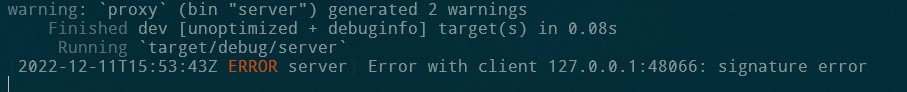
\includegraphics[width=\textwidth]{sig.jpg}
    \caption{代理服务器 Log}
    \label{fig:wrong-cred}
  \end{figure}

  \appendix
  \section{访问 Google 日志}
  \label{result:google}

  客户端的 Log 见图 \ref{fig:client-google}

  \begin{figure}
    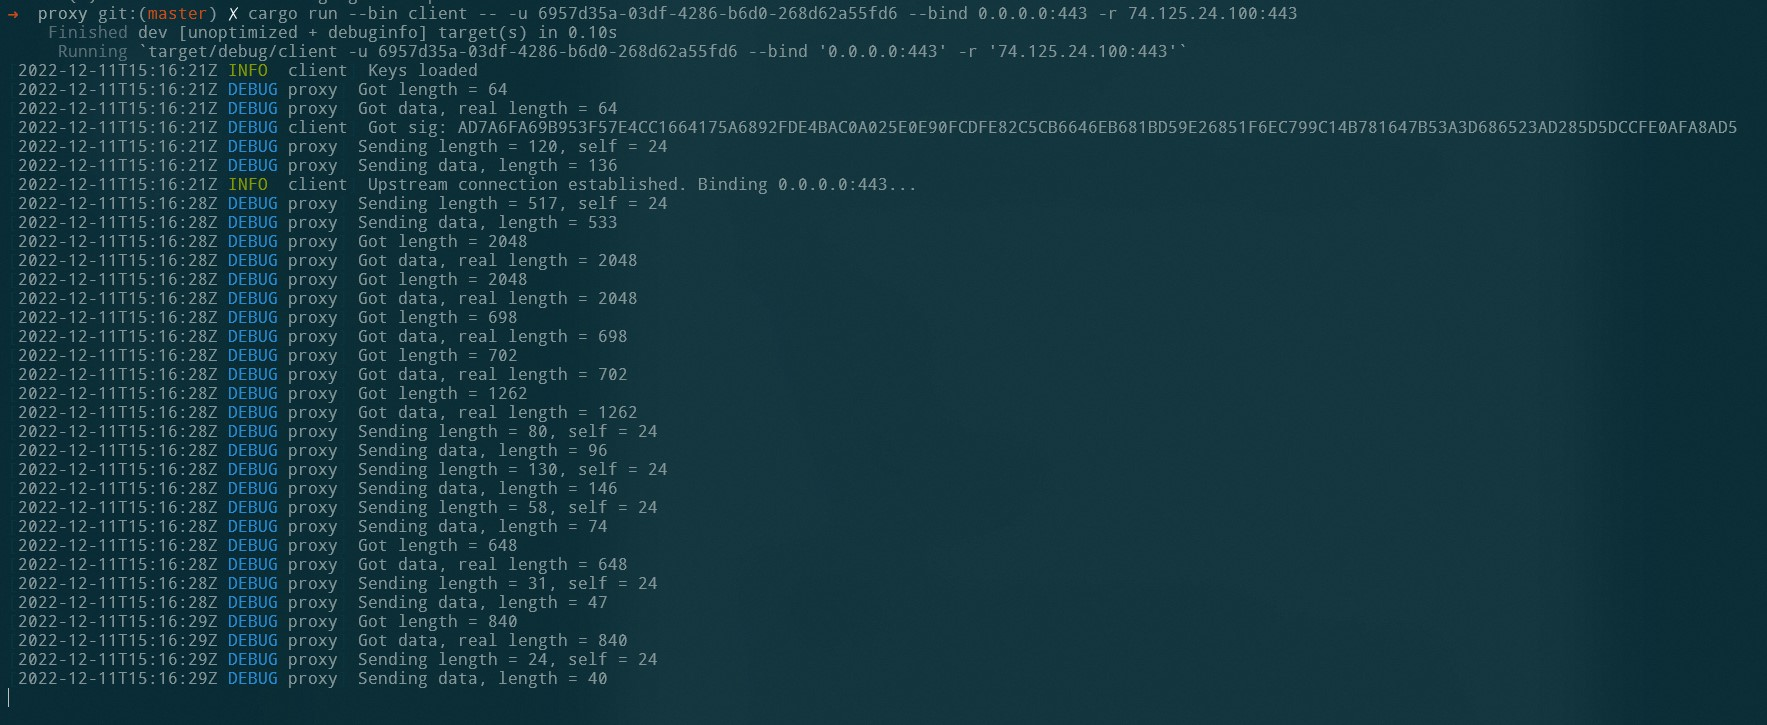
\includegraphics[width=\textwidth]{client-log-google.jpg}
    \caption{代理客户端 Log}
    \label{fig:client-google}
  \end{figure}

  curl log 为:

  \inputminted[]{text}{curl-log-google.txt}

  \section{访问 Google 日志}
  \label{result:google}
\end{document}